\documentclass[landscape]{article}
\usepackage[a3paper,margin=1cm]{geometry}
\usepackage[table]{xcolor}
\usepackage{tikz}
\usetikzlibrary{shapes.geometric, arrows.meta, positioning, fit, calc}

\definecolor{pkcolor}{RGB}{255,200,100}
\definecolor{fkcolor}{RGB}{150,200,255}
\definecolor{headercolor}{RGB}{70,130,180}
\definecolor{tablecolor}{RGB}{245,245,250}

\tikzset{
    table/.style={
        rectangle, draw=black, thick,
        minimum width=3.5cm, align=left,
        rounded corners=2pt
    },
    relation/.style={
        -Stealth, thick, gray!70
    }
}

\newcommand{\dbtable}[3]{
    % #1 = node name, #2 = position, #3 = content
    \node[table] (#1) #2 {
        \begin{tabular}{@{}l@{}}
        \rowcolor{headercolor}
        \textcolor{white}{\textbf{#3}}
        \end{tabular}
    };
}

\begin{document}
\pagestyle{empty}

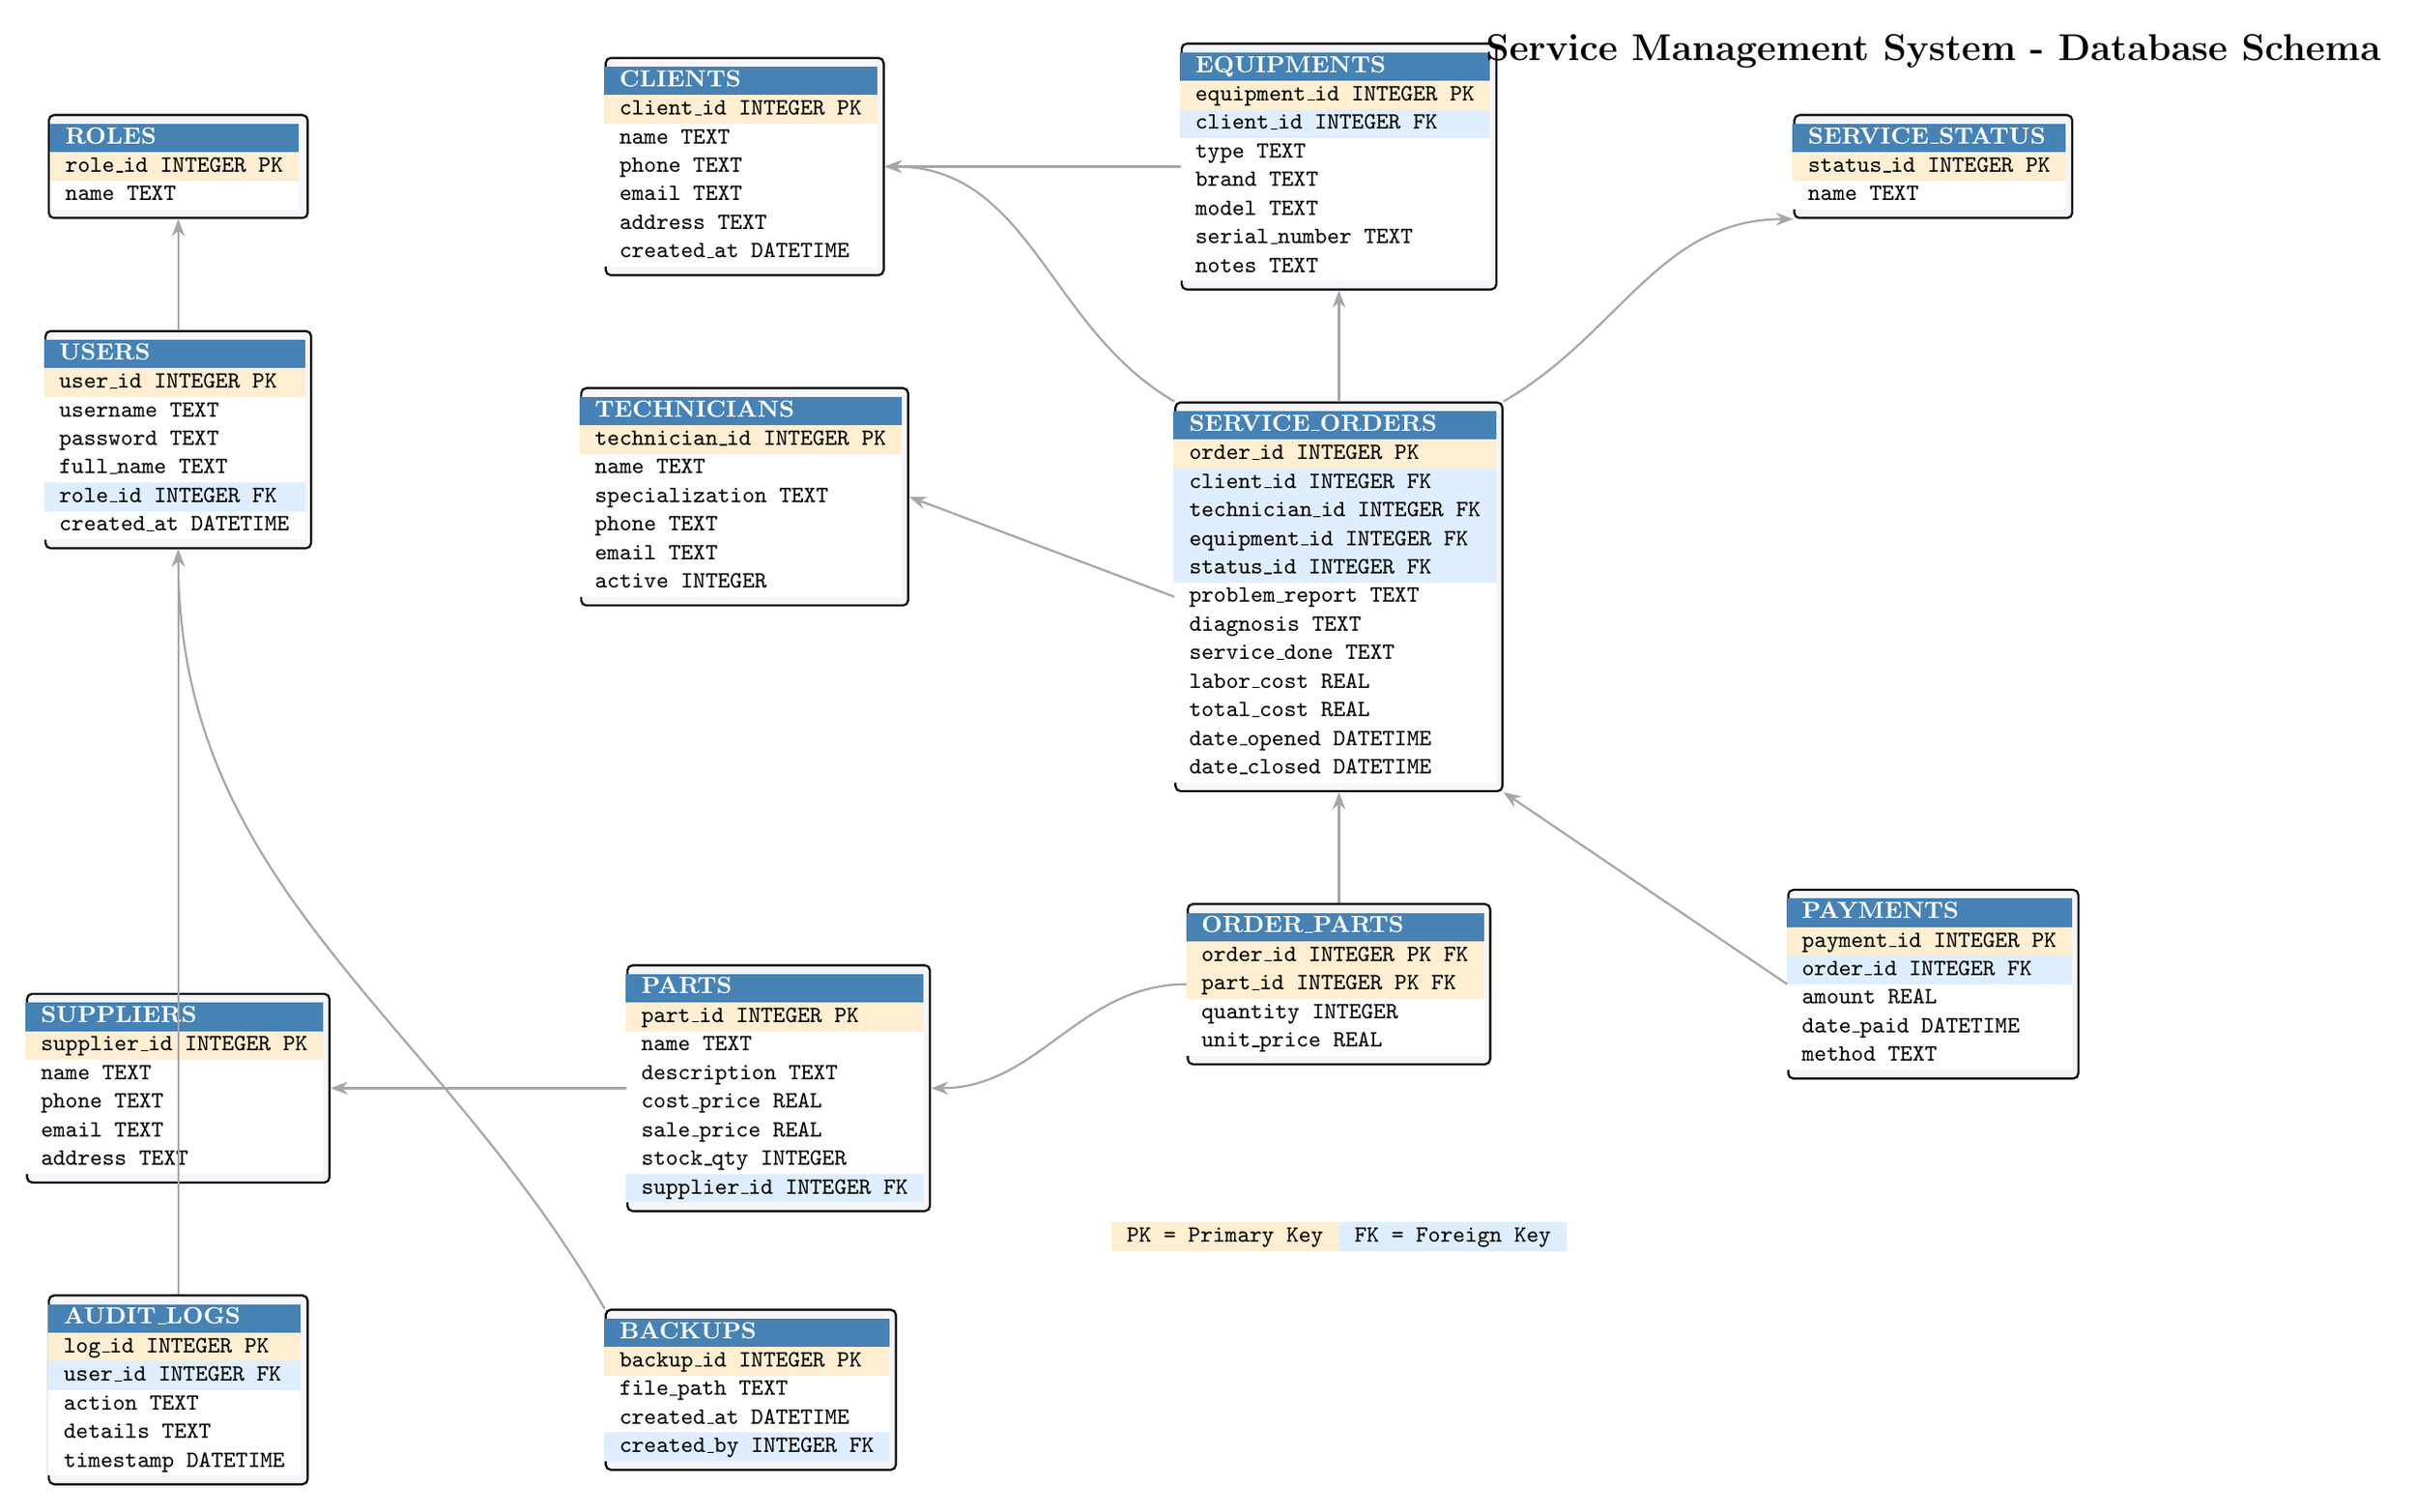
\begin{tikzpicture}[node distance=0.3cm, every node/.style={font=\small}]

% ============= AUTHENTICATION GROUP =============
\node[table, fill=tablecolor] (roles) at (0,0) {
    \begin{tabular}{@{\hspace{2pt}}l@{\hspace{2pt}}}
    \rowcolor{headercolor} \textcolor{white}{\textbf{ROLES}} \\
    \rowcolor{pkcolor!30} \ttfamily role\_id INTEGER PK \\
    \rowcolor{white} \ttfamily name TEXT \\
    \end{tabular}
};

\node[table, fill=tablecolor, below=1.5cm of roles] (users) {
    \begin{tabular}{@{\hspace{2pt}}l@{\hspace{2pt}}}
    \rowcolor{headercolor} \textcolor{white}{\textbf{USERS}} \\
    \rowcolor{pkcolor!30} \ttfamily user\_id INTEGER PK \\
    \rowcolor{white} \ttfamily username TEXT \\
    \rowcolor{white} \ttfamily password TEXT \\
    \rowcolor{white} \ttfamily full\_name TEXT \\
    \rowcolor{fkcolor!30} \ttfamily role\_id INTEGER FK \\
    \rowcolor{white} \ttfamily created\_at DATETIME \\
    \end{tabular}
};

% ============= CLIENTS/TECHNICIANS GROUP =============
\node[table, fill=tablecolor, right=4cm of roles] (clients) {
    \begin{tabular}{@{\hspace{2pt}}l@{\hspace{2pt}}}
    \rowcolor{headercolor} \textcolor{white}{\textbf{CLIENTS}} \\
    \rowcolor{pkcolor!30} \ttfamily client\_id INTEGER PK \\
    \rowcolor{white} \ttfamily name TEXT \\
    \rowcolor{white} \ttfamily phone TEXT \\
    \rowcolor{white} \ttfamily email TEXT \\
    \rowcolor{white} \ttfamily address TEXT \\
    \rowcolor{white} \ttfamily created\_at DATETIME \\
    \end{tabular}
};

\node[table, fill=tablecolor, below=1.5cm of clients] (technicians) {
    \begin{tabular}{@{\hspace{2pt}}l@{\hspace{2pt}}}
    \rowcolor{headercolor} \textcolor{white}{\textbf{TECHNICIANS}} \\
    \rowcolor{pkcolor!30} \ttfamily technician\_id INTEGER PK \\
    \rowcolor{white} \ttfamily name TEXT \\
    \rowcolor{white} \ttfamily specialization TEXT \\
    \rowcolor{white} \ttfamily phone TEXT \\
    \rowcolor{white} \ttfamily email TEXT \\
    \rowcolor{white} \ttfamily active INTEGER \\
    \end{tabular}
};

% ============= EQUIPMENT =============
\node[table, fill=tablecolor, right=4cm of clients] (equipments) {
    \begin{tabular}{@{\hspace{2pt}}l@{\hspace{2pt}}}
    \rowcolor{headercolor} \textcolor{white}{\textbf{EQUIPMENTS}} \\
    \rowcolor{pkcolor!30} \ttfamily equipment\_id INTEGER PK \\
    \rowcolor{fkcolor!30} \ttfamily client\_id INTEGER FK \\
    \rowcolor{white} \ttfamily type TEXT \\
    \rowcolor{white} \ttfamily brand TEXT \\
    \rowcolor{white} \ttfamily model TEXT \\
    \rowcolor{white} \ttfamily serial\_number TEXT \\
    \rowcolor{white} \ttfamily notes TEXT \\
    \end{tabular}
};

% ============= SERVICE ORDERS =============
\node[table, fill=tablecolor, right=4cm of equipments] (service_status) {
    \begin{tabular}{@{\hspace{2pt}}l@{\hspace{2pt}}}
    \rowcolor{headercolor} \textcolor{white}{\textbf{SERVICE\_STATUS}} \\
    \rowcolor{pkcolor!30} \ttfamily status\_id INTEGER PK \\
    \rowcolor{white} \ttfamily name TEXT \\
    \end{tabular}
};

\node[table, fill=tablecolor, below=1.5cm of equipments] (service_orders) {
    \begin{tabular}{@{\hspace{2pt}}l@{\hspace{2pt}}}
    \rowcolor{headercolor} \textcolor{white}{\textbf{SERVICE\_ORDERS}} \\
    \rowcolor{pkcolor!30} \ttfamily order\_id INTEGER PK \\
    \rowcolor{fkcolor!30} \ttfamily client\_id INTEGER FK \\
    \rowcolor{fkcolor!30} \ttfamily technician\_id INTEGER FK \\
    \rowcolor{fkcolor!30} \ttfamily equipment\_id INTEGER FK \\
    \rowcolor{fkcolor!30} \ttfamily status\_id INTEGER FK \\
    \rowcolor{white} \ttfamily problem\_report TEXT \\
    \rowcolor{white} \ttfamily diagnosis TEXT \\
    \rowcolor{white} \ttfamily service\_done TEXT \\
    \rowcolor{white} \ttfamily labor\_cost REAL \\
    \rowcolor{white} \ttfamily total\_cost REAL \\
    \rowcolor{white} \ttfamily date\_opened DATETIME \\
    \rowcolor{white} \ttfamily date\_closed DATETIME \\
    \end{tabular}
};

% ============= PARTS/INVENTORY =============
\node[table, fill=tablecolor, below=6cm of users] (suppliers) {
    \begin{tabular}{@{\hspace{2pt}}l@{\hspace{2pt}}}
    \rowcolor{headercolor} \textcolor{white}{\textbf{SUPPLIERS}} \\
    \rowcolor{pkcolor!30} \ttfamily supplier\_id INTEGER PK \\
    \rowcolor{white} \ttfamily name TEXT \\
    \rowcolor{white} \ttfamily phone TEXT \\
    \rowcolor{white} \ttfamily email TEXT \\
    \rowcolor{white} \ttfamily address TEXT \\
    \end{tabular}
};

\node[table, fill=tablecolor, right=4cm of suppliers] (parts) {
    \begin{tabular}{@{\hspace{2pt}}l@{\hspace{2pt}}}
    \rowcolor{headercolor} \textcolor{white}{\textbf{PARTS}} \\
    \rowcolor{pkcolor!30} \ttfamily part\_id INTEGER PK \\
    \rowcolor{white} \ttfamily name TEXT \\
    \rowcolor{white} \ttfamily description TEXT \\
    \rowcolor{white} \ttfamily cost\_price REAL \\
    \rowcolor{white} \ttfamily sale\_price REAL \\
    \rowcolor{white} \ttfamily stock\_qty INTEGER \\
    \rowcolor{fkcolor!30} \ttfamily supplier\_id INTEGER FK \\
    \end{tabular}
};

\node[table, fill=tablecolor, below=1.5cm of service_orders] (order_parts) {
    \begin{tabular}{@{\hspace{2pt}}l@{\hspace{2pt}}}
    \rowcolor{headercolor} \textcolor{white}{\textbf{ORDER\_PARTS}} \\
    \rowcolor{pkcolor!30} \ttfamily order\_id INTEGER PK FK \\
    \rowcolor{pkcolor!30} \ttfamily part\_id INTEGER PK FK \\
    \rowcolor{white} \ttfamily quantity INTEGER \\
    \rowcolor{white} \ttfamily unit\_price REAL \\
    \end{tabular}
};

% ============= PAYMENTS =============
\node[table, fill=tablecolor, right=4cm of order_parts] (payments) {
    \begin{tabular}{@{\hspace{2pt}}l@{\hspace{2pt}}}
    \rowcolor{headercolor} \textcolor{white}{\textbf{PAYMENTS}} \\
    \rowcolor{pkcolor!30} \ttfamily payment\_id INTEGER PK \\
    \rowcolor{fkcolor!30} \ttfamily order\_id INTEGER FK \\
    \rowcolor{white} \ttfamily amount REAL \\
    \rowcolor{white} \ttfamily date\_paid DATETIME \\
    \rowcolor{white} \ttfamily method TEXT \\
    \end{tabular}
};

% ============= LOGS/BACKUPS =============
\node[table, fill=tablecolor, below=1.5cm of suppliers] (audit_logs) {
    \begin{tabular}{@{\hspace{2pt}}l@{\hspace{2pt}}}
    \rowcolor{headercolor} \textcolor{white}{\textbf{AUDIT\_LOGS}} \\
    \rowcolor{pkcolor!30} \ttfamily log\_id INTEGER PK \\
    \rowcolor{fkcolor!30} \ttfamily user\_id INTEGER FK \\
    \rowcolor{white} \ttfamily action TEXT \\
    \rowcolor{white} \ttfamily details TEXT \\
    \rowcolor{white} \ttfamily timestamp DATETIME \\
    \end{tabular}
};

\node[table, fill=tablecolor, right=4cm of audit_logs] (backups) {
    \begin{tabular}{@{\hspace{2pt}}l@{\hspace{2pt}}}
    \rowcolor{headercolor} \textcolor{white}{\textbf{BACKUPS}} \\
    \rowcolor{pkcolor!30} \ttfamily backup\_id INTEGER PK \\
    \rowcolor{white} \ttfamily file\_path TEXT \\
    \rowcolor{white} \ttfamily created\_at DATETIME \\
    \rowcolor{fkcolor!30} \ttfamily created\_by INTEGER FK \\
    \end{tabular}
};

% ============= RELATIONSHIPS =============
% Authentication
\draw[relation] (users.north) -- (roles.south);

% Equipments
\draw[relation] (equipments.west) -- (clients.east);

% Service Orders
\draw[relation] (service_orders.north) -- (equipments.south);
\draw[relation] (service_orders.west) -- (technicians.east);
\draw[relation] (service_orders.north west) to[out=150,in=0] (clients.east);
\draw[relation] (service_orders.north east) to[out=30,in=180] (service_status.south west);

% Order Parts
\draw[relation] (order_parts.north) -- (service_orders.south);
\draw[relation] (order_parts.west) to[out=180,in=0] (parts.east);

% Parts
\draw[relation] (parts.west) -- (suppliers.east);

% Payments
\draw[relation] (payments.west) -- (service_orders.south east);

% Logs
\draw[relation] (audit_logs.north) to[out=90,in=270] (users.south);
\draw[relation] (backups.north west) to[out=120,in=270] (users.south);

% ============= LEGEND =============
\node[below=2cm of order_parts, anchor=north, font=\small] (legend) {
    \begin{tabular}{cc}
    \cellcolor{pkcolor!30}\ttfamily PK = Primary Key & 
    \cellcolor{fkcolor!30}\ttfamily FK = Foreign Key \\
    \end{tabular}
};

% Title
\node[above=0.5cm of service_status, font=\Large\bfseries] {Service Management System - Database Schema};

\end{tikzpicture}

\end{document}